\documentclass[12pt,a4paper]{article}
% The following LaTeX packages must be installed on your machine: amsmath, authblk, bm, booktabs, caption, dcolumn, fancyhdr, geometry, graphicx, hyperref, latexsym, natbib
\input{183.dat}
\usepackage{gensymb}
\usepackage{amsthm}
\usepackage{float}
\usepackage{siunitx}
\usepackage{amssymb}
\usepackage{float}
\usepackage{enumerate}
\usepackage{listings}
\usepackage{mathtools}
\PassOptionsToPackage{hyphens}{url}\usepackage{hyperref}
\usepackage[none]{hyphenat}
\usepackage{physics}
\newcommand\ddfrac[2]{\frac{\displaystyle #1}{\displaystyle #2}}
%\renewcommand{\familydefault}{\sfdefault}


\begin{document}

\setcounter{page}{1}

\section*{Lead Compensation}
\bigskip

With student number 03116, the transfer function is

\begin{equation}
	G(s) = \frac{3}{s^2 + s} \label{eq:transfer-func}
\end{equation}

\noindent
with a desired peak at 0.25 s after excitation with an overshoot of no more than 40\%. The overall transfer function of \eqref{eq:transfer-func} in a unity gain negative feedback is

\begin{equation}
	H(s) = \frac{G(s)}{1 + G(s)} \label{eq:negative-feedback}
\end{equation}

\begin{figure}[h!]
	\centering
	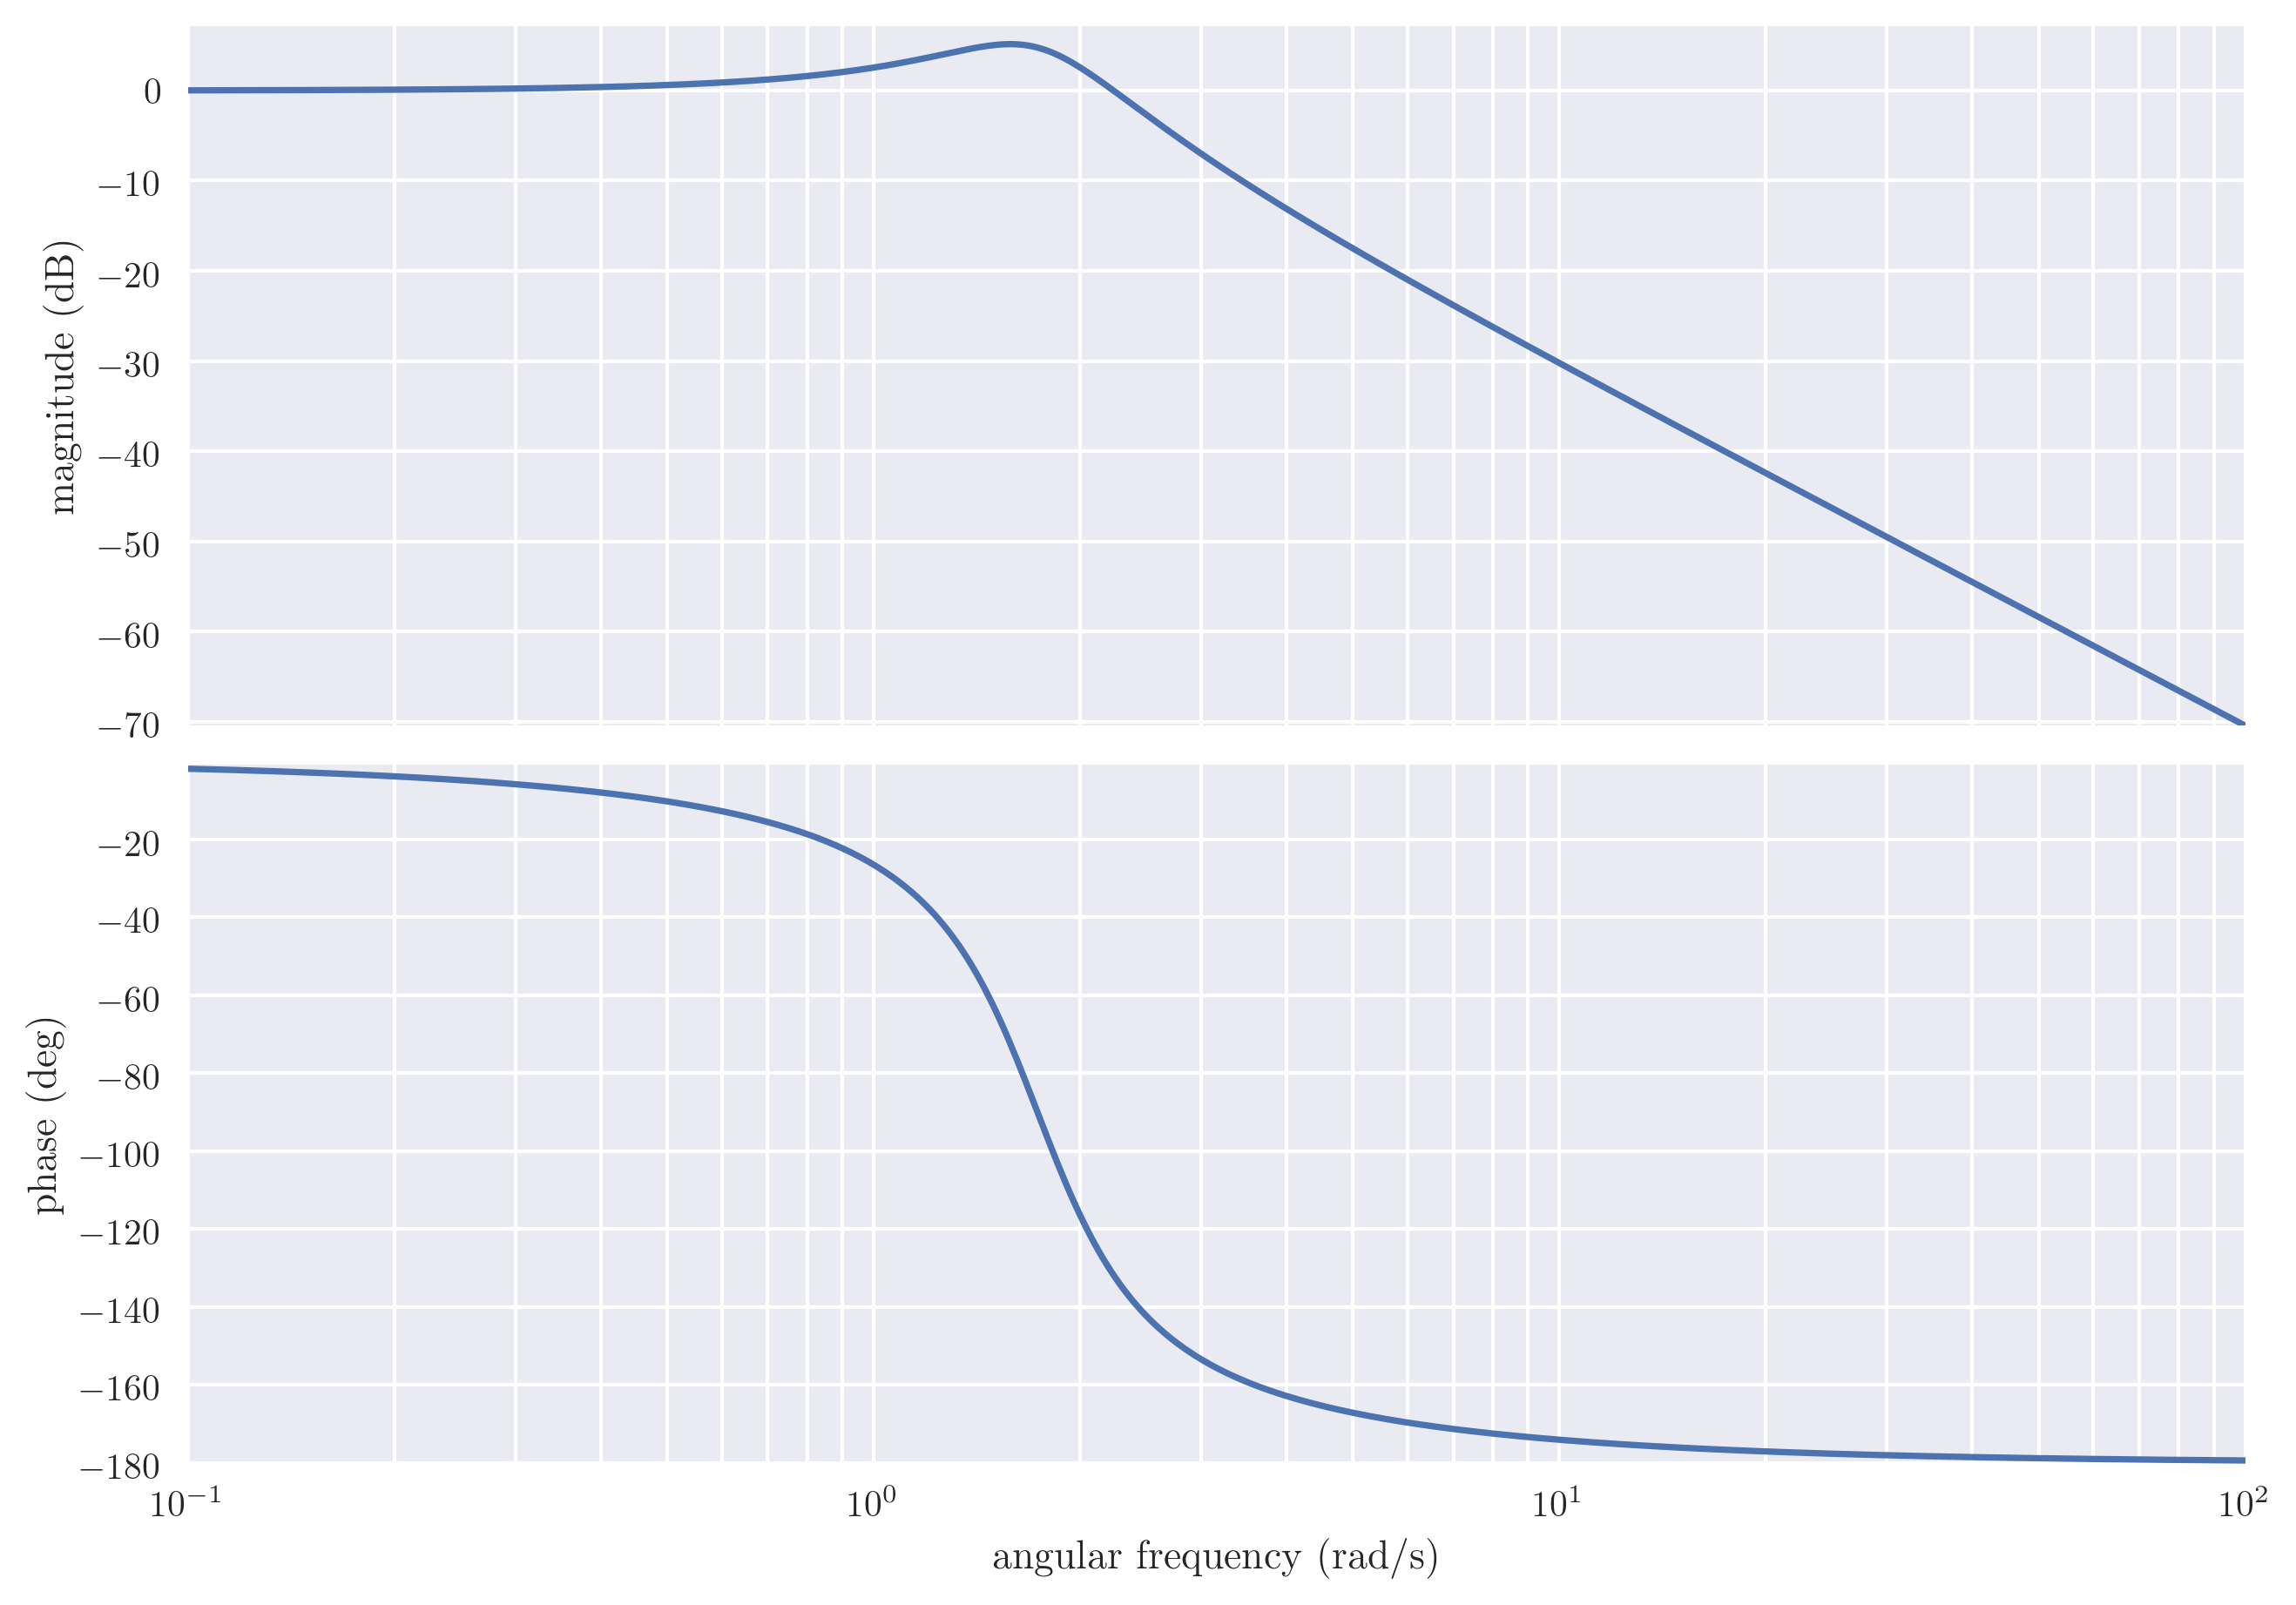
\includegraphics[width=0.7\linewidth]{sys_bode.png}
	\caption{Bode plot of \eqref{eq:negative-feedback}.}
	\label{fig:bode}
\end{figure}

\begin{figure}[h!]
	\centering
	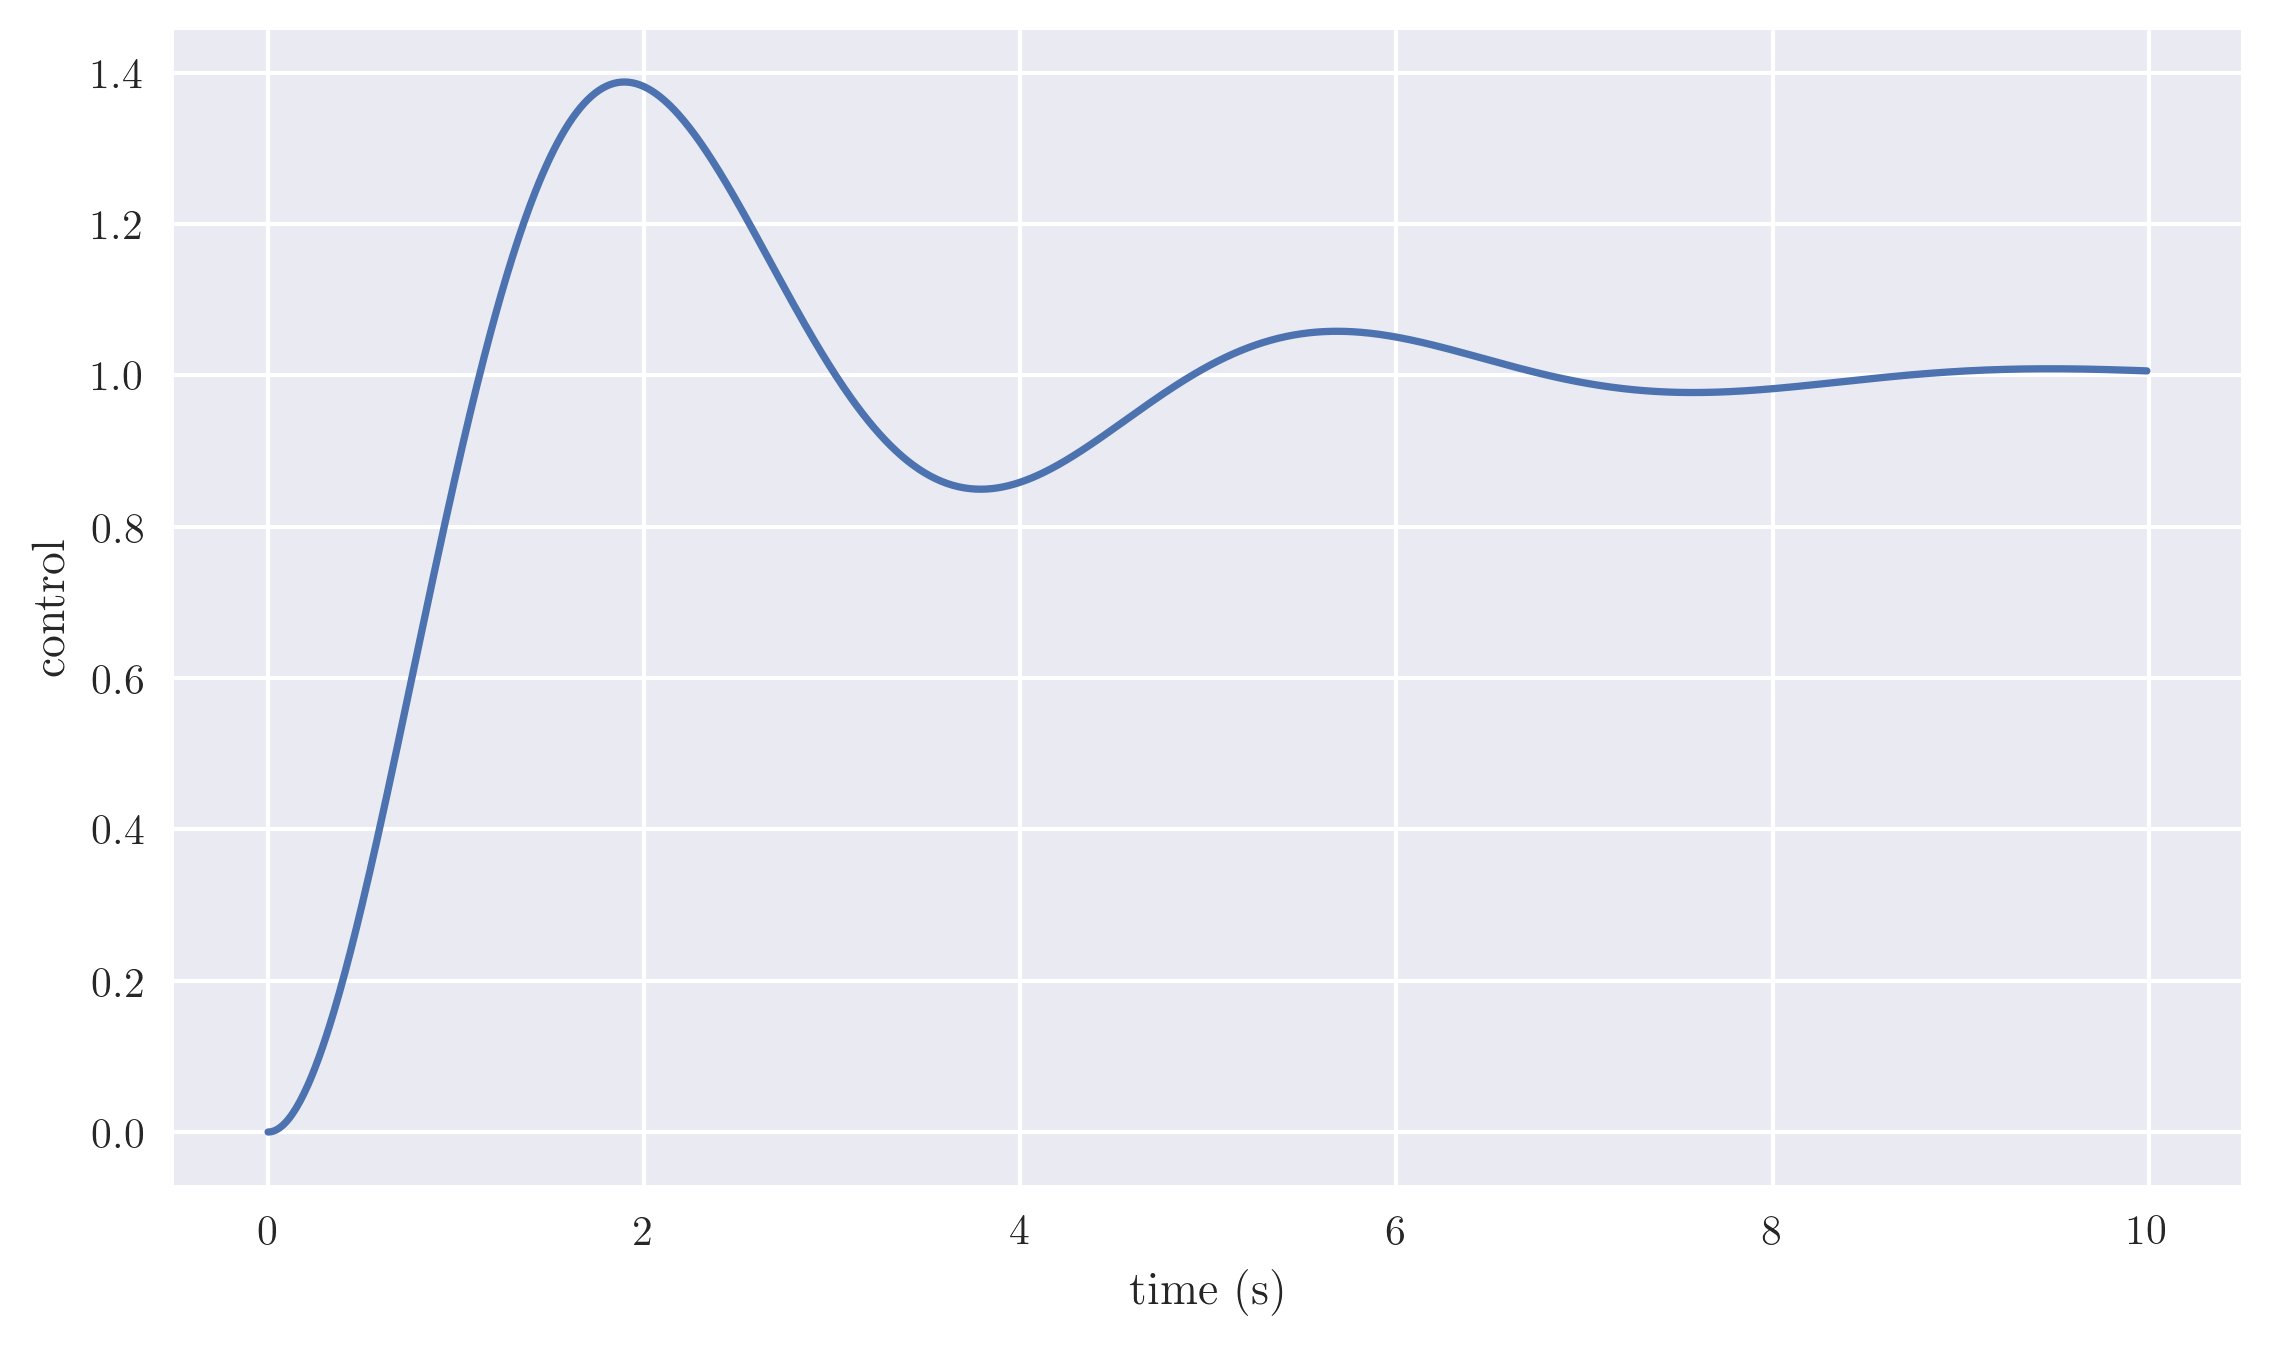
\includegraphics[width=0.7\linewidth]{sys-response.png}
	\caption{Step function response of \eqref{eq:negative-feedback}.}
	\label{fig:sys-response}
\end{figure}

\begin{enumerate}[(a)]

\item \textbf{Desired pole location}

\begin{align}
	s_d &= -\sigma_d \pm j\omega_d \\
	&= -\zeta\omega_n + j\omega_n \sqrt{1-\zeta^2} \\
	\zeta &= \frac{-\ln(\%OS)}{\sqrt{\pi^2 + \ln^2(\%OS)}} \\
	&= \frac{-\ln(0.4)}{\sqrt{\pi^2 + \ln^2(0.4)}} \\
	\Aboxed{
		\zeta &= 0.28
	} \label{eq:zeta} \\
	\omega_n &= \frac{\pi}{T_p \sqrt{1-\zeta^2}} \\
	&= \frac{\pi}{0.25\sqrt{1-0.28^2}} \\
	\Aboxed{
		\omega_n &= 13.09
	} \label{eq:natural-freq} \\
	\Aboxed{
		s_d &= -3.67 + 12.57j
	} \label{eq:desired-pole}
\end{align}

\item \textbf{Angle deficiency}

\begin{align}
	G(s_d) &= \frac{3}{s_d^2 + s_d} \\
	&= -0.02 + 0.01j \\
	\measuredangle G(s_d) &= 203.81^\circ \\
	\Phi_d &= 180 - \measuredangle G(s_d) \\
	\Aboxed{
		\Phi_d &= 0.49 \textrm{ rad} = 28.23^\circ
	} \label{eq:angle-def}
\end{align}

\item \textbf{Compensator poles and zeros}

\begin{align}
	\alpha &= \arctan(\frac{\sqrt{1-\zeta^2}}{\zeta}) \\
	&= \arctan(\frac{\sqrt{1-0.28^2}}{0.28}) \\
	\Aboxed{
		\alpha &= 1.29
	} \label{eq:alpha} \\
	z_c &= -\omega_n \sqrt{1-\zeta^2} \tan(\frac{\alpha - \Phi_d}{2}) - \zeta\omega_n \\
	&= -(13.09)\sqrt{1-0.28^2}\tan(\frac{1.29 - 0.49}{2}) - (0.28)(13.09) \\
	\Aboxed{
		z_c &= -8.94
	} \label{eq:compensator-zero} \\
	p_c &= -\omega_n \sqrt{1-\zeta^2} \tan(\frac{\alpha + \Phi_d}{2}) - \zeta\omega_n \\
	&= -(13.09)\sqrt{1-0.28^2}\tan(\frac{1.29 + 0.49}{2}) - (0.28)(13.09) \\
	\Aboxed{
		p_c &= -19.18
	} \label{eq:compensator-pole}
\end{align}

\item \textbf{Compensator gain}

\begin{align}
	K_c &= \ddfrac{1}{\abs{G(s_d)\frac{s_d + p_c}{s_d + z_c}}} \\
	&= \ddfrac{1}{\abs{-0.02 + 0.01j \frac{-3.67 + 12.57j - 8.94}{-3.67 + 12.57j - 19.18}}} \\
	\Aboxed{
		K_c &= 82.11
	} \label{eq:compensator-gain}
\end{align}

\item \textbf{Simulink verification}

\begin{figure}[h!]
	\centering
	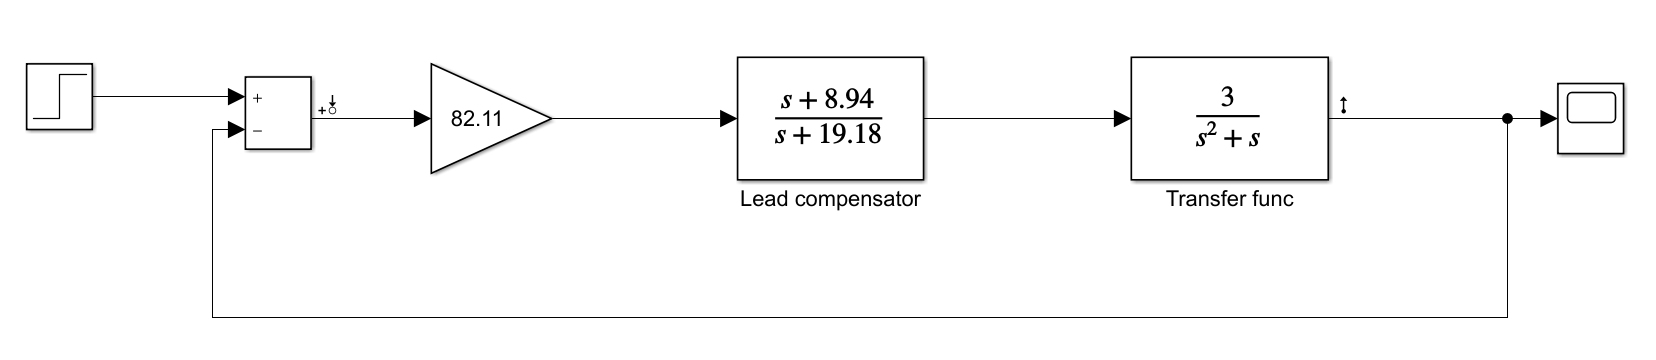
\includegraphics[width=0.9\linewidth]{compensator-design.png}
	\caption{Block diagram design of \eqref{eq:negative-feedback} with a lead compensator.}
	\label{fig:comp-design}
\end{figure}

\begin{figure}[h!]
	\centering
	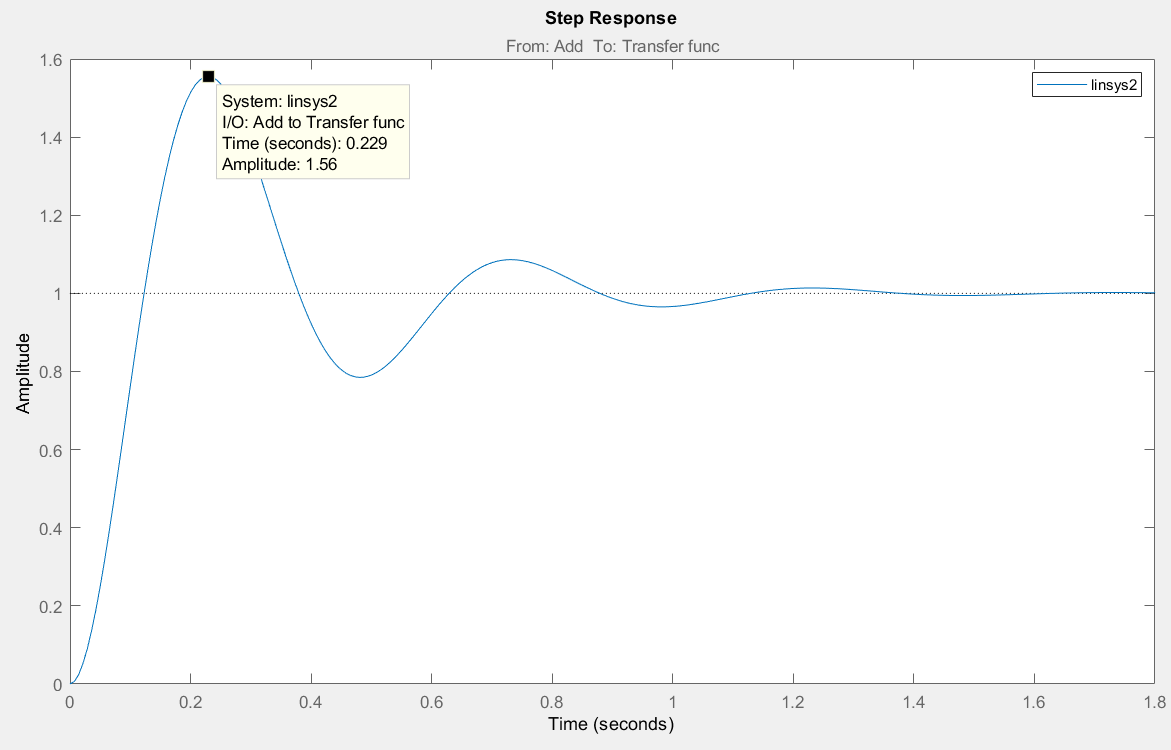
\includegraphics[width=0.9\linewidth]{compensator-step.png}
	\caption{Step function response of the system with a lead compensator. Due to rounding-off errors, the peak time occurs at  $t = 0.229$ s.}
	\label{fig:comp-design}
\end{figure}

\begin{figure}[h!]
	\centering
	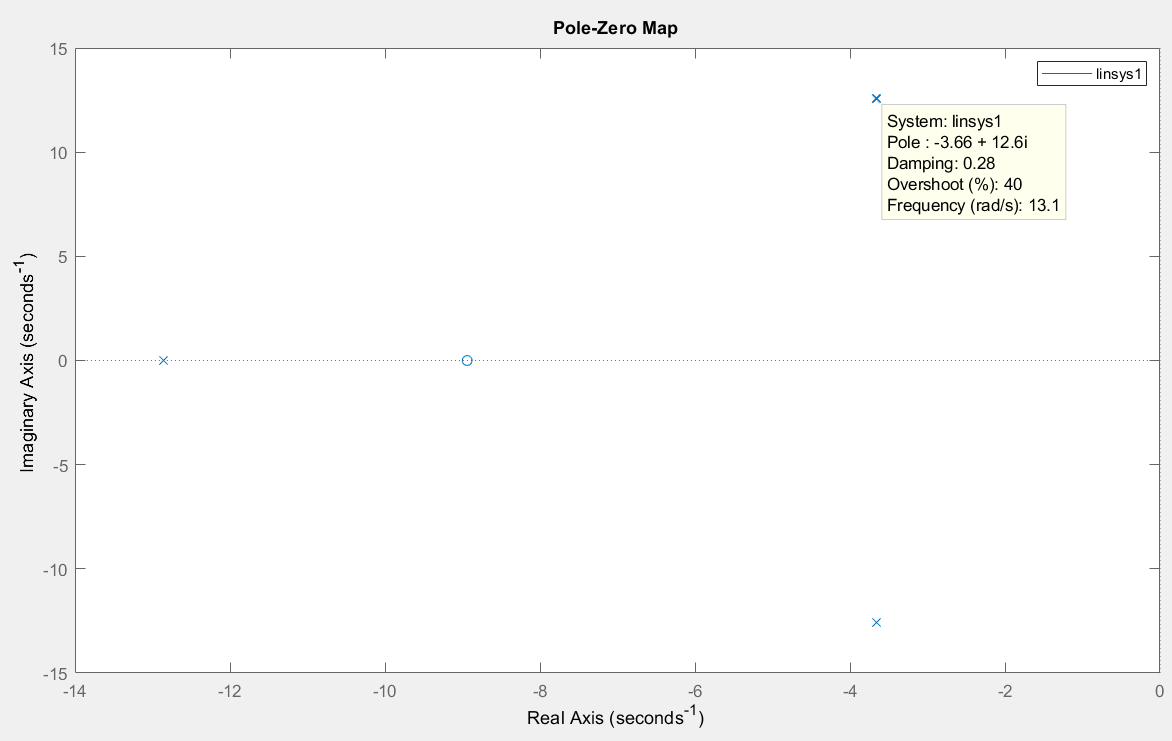
\includegraphics[width=0.9\linewidth]{compensator-pole.png}
	\caption{Pole-zero map of the system with a lead compensator. The percent overshoot is exactly 40\%.}
	\label{fig:comp-design}
\end{figure}

\end{enumerate}

\clearpage

\section*{Appendix}

\lstset{
	basicstyle=\footnotesize\ttfamily,
	language=Python,
	tabsize=4,
	numbers=left,
	numberstyle=\tiny\ttfamily,
	caption={Source code.},
	label=list:source
}
\begin{lstlisting}
import numpy as np
import matplotlib.pyplot as mp
import matplotlib.ticker as tick


class LeadCompensator:
    
    def __init__(self, w):
        self.w = w
        self.s = 1j*w
        
    def initTransferFunc(self, G):
        self.G = G
        
    def initNegativeFeedback(self, gain):
        self.k = gain
        self.H = self.G(self.s)/(1 + self.k*self.G(self.s))
        self.magnitude = 20*np.log10(self.H)
        self.phase = np.degrees(np.arctan2(self.H.imag, self.H.real))
        
    def BodePlot(self, save=False, savename=None):
        fig = mp.figure(figsize=(5*16/9, 5*1.25))
        
        ax = fig.add_subplot(211)
        ax.plot(self.w, self.magnitude)
        ax.set_xscale("log")
        ax.grid(True, which="both")
        ax.set_ylabel("magnitude (dB)")
        ax.set_xlim(self.w.min(), self.w.max())
        ax.set_ylim(self.magnitude.min(), self.magnitude.max()+2)
        ax.xaxis.set_major_formatter(tick.NullFormatter())
        
        ax = fig.add_subplot(212)
        ax.plot(self.w, self.phase)
        ax.set_xscale("log")
        ax.grid(True, which="both")
        ax.set_xlabel("angular frequency (rad/s)")
        ax.set_ylabel("phase (deg)")
        ax.set_xlim(self.w.min(), self.w.max())
        ax.set_ylim(self.phase.min()-1, self.phase.max()+1)
        
        mp.tight_layout()
        if save:
            mp.savefig(savename, dpi=300, bbox_inches="tight")
        mp.show()
        
    def initDesired(self, percent_overshoot, Tp):
        self.zeta = -np.log(percent_overshoot)/np.sqrt(np.pi**2 + \
                                            np.log(percent_overshoot)**2)
        self.wn = np.pi/(Tp * np.sqrt(1 - self.zeta**2))
        self.sd = -self.zeta*self.wn + 1j*self.wn*np.sqrt(1 - self.zeta**2)
        self.Gsd = self.G(self.sd)
        phiGsd = np.arctan2(self.Gsd.imag, self.Gsd.real)
        self.phid = np.pi - phiGsd
        
    def initCompensator(self):
        self.alpha = np.arctan2(np.sqrt(1 - self.zeta**2), self.zeta)
        self.zc = -self.wn*np.sqrt(1 - self.zeta**2) * \
                    np.tan((self.alpha - self.phid)/2) - self.zeta*self.wn
        self.pc = -self.wn*np.sqrt(1 - self.zeta**2) * \
                    np.tan((self.alpha + self.phid)/2) - self.zeta*self.wn
        self.K = 1/abs(self.Gsd*(self.sd + self.zc)/(self.sd + self.pc))
        
def G(s):
	return 3/(s**2 + s)
	
w = np.logspace(-1, 2, 500)
sys = LeadCompensator(w)
sys.initTransferFunc(G)
sys.initNegativeFeedback(1)
sys.BodePlot(True, "sys_bode.png")
sys.initDesired(0.4, 0.25)
sys.initCompensator()
\end{lstlisting}

\end{document}